\documentclass[../main.tex]{subfiles}

\begin{document}

\subsection*{Exercice 1 : Représentation d'état de correcteurs analogiques}

\noindent 1- Correcteur à avance de phase
On considère le circuit suivant :

\noindent a) Établissons les différentes relations entrée sorties de chaque composants:\\
\begin{itemize}
\item $u = Ri$
\item $u_2 = R_2i_2$
\item $ u_1 = R_1i_1$
\item $u_3 = R_3i_3$
\item $ i_c = C\frac{d u_c}{dt}$
\end{itemize}
\bigbreak

On se propose ensuite de construire un modèle d'état de vecteur d'état $x \in \mathbb{R^n}$ tel que : $\dot{x}(t)= Ax(t) + B e(t)$ équation d'état.\\
Équation d'observation : $s(t) = Cx(t) + De(t)$\\

La loi des nœuds donne :
\begin{itemize}
\item $ i_2 = i_1+i_3$
\item $ i = i_2$
\item $ i_c = i_3$
\end{itemize}
\bigbreak

La loi des mailles donne :
\begin{itemize}
\item $e = u$
\item $ u_2 + u_1 + s = 0$
\item $ u_2 + u_3 + u_c = 0$
\end{itemize}

On obtient en recoupant judicieusement l'équation d'état : \\
$ \dot{u_C} = \frac{-1}{R_3C}u_C - \frac{R_2}{RR_3}e = Au_C + B e$\\
Et l'équation d'observation : $s = \frac{-R_1}{R_3}u_C - (\frac{R_1R_2}{RR_3}+\frac{R_1+R_2}{R})e =  Cu_C + De$

\noindent 2 et 3 à faire .

\subsection*{Exercice 2 : association de systèmes}

On considère les deux systèmes (S1) et (S2) respectivement décrits par les représentation d'état :
\begin{align*}
(S1)\left \{ \begin{matrix}
\dot{x_1} = A_1x_1 + B_1u_1\\
y_1 = C_1x_1 + D_1 u_1
\end{matrix} \right.\\
(S2)\left \{ \begin{matrix}
\dot{x_2} = A_2x_2 + B_2u_2\\
y_2 = C_2x_2 + D_2 u_2
\end{matrix} \right.
\end{align*}
\begin{enumerate}

\item On place les deux systèmes (S1) et (S2) en série selon le schéma suivant :
\begin{center}
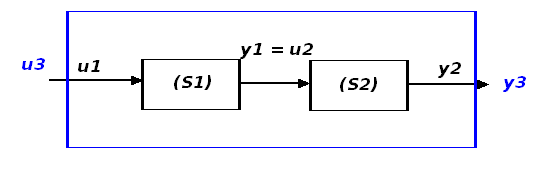
\includegraphics[scale=0.5]{TD5-1.png}
\end{center}

On a donc la relation de connections : $y_1 = u_2$.\\
On en déduit les relations de connections suivantes :
\begin{align*}
\dot{x_2} &= A_2x_2+B_2(C_1x_1+D_1u_1)\\
y_2 &= C_2x_2+D_2(C_1x_1+D_1u_1)\\
\dot{x_1} &= A_1x_1+B_1u_1\\
\end{align*}

On obtient donc l'équation d'état suivante :\\
\begin{align*}
\begin{pmatrix}
\dot{x_1}\\\dot{x_2}\end{pmatrix} &= \begin{pmatrix}
A_1&0\\B_2C_1 & A_2\end{pmatrix}.\begin{pmatrix}
x_1\\x_2\end{pmatrix} + \begin{pmatrix}
B_1\\B_2D_1\end{pmatrix} u_1
\intertext{On pose donc :}
x_3 &= \begin{pmatrix}\dot{x_1}\\\dot{x_2}\end{pmatrix}
\intertext{Et on a donc comme équation d'observation avec $y_3 = y_2$}
y_3 &= \begin{pmatrix}
D_2C_1 & C_2\end{pmatrix} x_3 +D_2D_1 u_1
\end{align*}


\item On place ensuite (S1) et (S2) en parallèle selon le schéma suivant :
\begin{center}
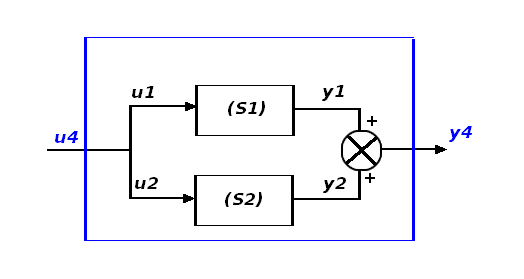
\includegraphics[scale=0.5]{TD5-2.png}
\end{center}
On a donc comme relations de connections :
\begin{align*}
u_4 &= u_1 = u_2\\
y_4 &= y_2 + y_4
\end{align*}

On veut comme équation d'état une forme : $\dot{x_4} = A_4 x_4 + B_4 u_4$, avec $x_4$ à déterminer.\\
Comme on a $\dot{x_1} = A_1x_1 + B_1u_1$ et $\dot{x_2} = A_2x_2 + B_2u_2$, et que $u_4 = u_1 = u_2$. On peut directement se ramener à :
\begin{align*}
\begin{pmatrix}
\dot{x_1}\\\dot{x_2}\end{pmatrix} &= \begin{pmatrix}
A_1&0\\0&A_2\end{pmatrix}.\begin{pmatrix}
x_1\\x_2\end{pmatrix} + \begin{pmatrix}
B_1\\B_2\end{pmatrix} u_4\\
&=A_4 x_4 + B_4 u_4
\intertext{En posant $x_4 =\begin{pmatrix}
x_1\\x_2\end{pmatrix}$ }
\intertext{De plus en sommant les equations sur $y_1$ et $y_2$ :}
y_4 &= C_1x_1 + C_2 x_2 + (D_1 + D_2) u_4\\
&= \begin{pmatrix}
C_1&C_2\end{pmatrix}.\begin{pmatrix}
x_1\\x_2\end{pmatrix} + (D_1+D_2)u_4\\
&= C_4 x_4 + D_4 u_4
\end{align*}
On a donc une équation d'observation en $x_4$ et $y_4$

\item On asservie la structure (S3) précédente avec une retour unitaire comme sur le schéma suivant :\\
\begin{center}
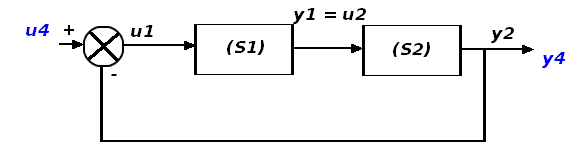
\includegraphics[scale=0.5]{TD5-3.png}
\end{center}
On a comme relation de connections :\\
\begin{align*}
u_3 &= u_5 -y_5\\
y_3 &= y_5
\intertext{on a donc en remplaçant dans l'équation d'observation du système 3 :}
y_5 &= C_3 x_3 + D_3(u_5 - y_5)
\intertext{ATTENTION! Dans el cas général ce sont des matrices et non commutable :}
(\mathbb{1} + D_3)y_5 &= C_3x_3 + D_3 u_5
\intertext{si $\mathbb{1}+ D_4$ est inversible :}
y_5 &= (\mathbb{1} + D_3)^{-1}C_3 x_3 + (\mathbb{1} + D_3)^{-1}D_3 u_5\\
&= C_5 x_3 + D_5 u_5
\end{align*}
On parle ici de boucle de rétroaction bien posée. Ceci est notre équation d'observation si $x_3 = x_5$.\\
Si l'on remplace dans l'équation d'état de (S3) :
\begin{align*}
\dot{x_3} &= A_3 x_3 + B_3(u_5 - y_5)\\
&= A_3 x_3 + B_3u_5 - B_3((\mathbb{1} + D_3)^{-1}C_3 x_3 + (\mathbb{1} + D_3)^{-1}D_3 u_5)\\
&= (A_3 - B_3(\mathbb{1} + D_3)^{-1}C_3)x_3 + B_3(\mathbb{1} - (\mathbb{1} + D_3)^{-1}D_3)u_5\\
&= A_5 x_5 + B_5 u_5
\end{align*}
On obtient donc l'équation d'état avec $x_5 = x_3$. Pour cette question, il ne reste plus qu'à exprimer les termes de (S3) en fonction de ceux de (S2) et (S1).\\

\item Dans celle-ci, on boucle le système (S4), il suffit donc de reprendre les mêmes calcules que dans la question précédent avec un changement d'indice. Il suffit ensuite d'exprimer les termes de (S4) en fonction de ceux de (S2) et (S1).\\

\item On place le système (S1) sur la chaine directe et (S2) sur la chaîne de retour comme le montre le schéma suivant :\\
\begin{center}
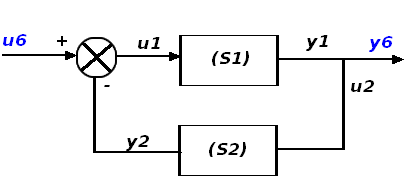
\includegraphics[scale=0.5]{TD5-4.png}
\end{center}
On a les deux relations de connections :\\
\begin{align*}
y_1 &= y_6 = u_2\\
u_1 &= u_6 - y_2
\end{align*}
Puisque l'on a une expression de $y_6$ directement depuis l'équation d'observation de (S1) :
\begin{align*}
y_6 &= y_1 = C_1 x_1 + D_1 (u_6 -y_2)\\
(\mathbb{1}+ D_1D_2)y_6 &= C_1x_1 + D_1C_2x_2 + D_1 u_6\\
\intertext{donc si $(\mathbb{1}+ D_1D_2)$ est inversible :}
y_6 &= (\mathbb{1}+ D_1D_2)^{-1} C_1 x_1 + (\mathbb{1}+ D_1D_2)^{-1}D_1C_2 x_2 + (\mathbb{1}+ D_1D_2)^{-1}D_1 u_6\\
&= \begin{pmatrix}
(\mathbb{1}+ D_1D_2)^{-1}C_1 & (\mathbb{1}+ D_1D_2)^{-1}D_1C_2\end{pmatrix}. \begin{pmatrix}
x_1\\x_2\end{pmatrix} + (\mathbb{1}+ D_1D_2)^{-1}D_1 u_6\\
&= C_6 x_6 + D_6 u_6
\end{align*}
On pose donc $x_6 = \begin{pmatrix}x_1\\x_2\end{pmatrix}$. Déterminons alors l'équation d'état composante par composante :
\begin{align*}
\dot{x_1} &= A_1 x_1 + B_1 u_1\\
&= A_1 x_1 +B_1(u_6 -y_2)\\
&= A_1 x_1  - B_1 C_2x_2 - B_1 D_2 y_6 + B_1 u_6\\
\intertext{En remplaçant par l'équation d'observation de (S6) :}
\dot{x_1}&= \begin{pmatrix}A_1& - B_1 C_2\end{pmatrix}x_6 - B_1 D_2 C_6 x_6 + (B_1-D_6) u_6
\intertext{Et pour la deuxième :}
\dot{x_2} &= A_2 x_2 + B_2u_2\\
&= A_2 x_2 +B_2 y_6\\
&= \begin{pmatrix}
A_1 - B_1C_2\end{pmatrix}x_6 + B_2D_6 u_6
\intertext{Ainsi, en recoupant ces deux composantes on a le système d'état :}
\dot{x_6} &= \begin{pmatrix}
A_1 + B_1D_2(\mathbb{1}+ D_1D_2)^{-1}C_1 & -B_1C_2-B_1D_2(\mathbb{1}+ D_1D_2)^{-1}D_1C_2\\
B_2(\mathbb{1}+ D_1D_2)^{-1}C_1 & A_2-B_2(\mathbb{1}+ D_1D_2)^{-1}D_1C_2
\end{pmatrix}x_6 + \begin{pmatrix}
B_1-(\mathbb{1}+ D_1D_2)^{-1}D_1\\
B_2(\mathbb{1}+ D_1D_2)^{-1}D_1
\end{pmatrix}u_6\\
&=A_6 x_6 + B_6 u_6
\end{align*}
Attention : résultat risqué.
\end{enumerate}



\end{document}
